\documentclass[11pt,a4paper]{article}

% --- Core Packages ---
\usepackage[utf8]{inputenc}
\usepackage[T1]{fontenc}
\usepackage[english]{babel}
\usepackage{geometry}
\usepackage{xcolor}
\usepackage{amsmath,amssymb,amsfonts,mathtools}
\usepackage{booktabs,tabularx,array,multirow}
\usepackage{listings}
\usepackage{tikz}
\usetikzlibrary{arrows.meta,positioning,shapes.geometric,trees,backgrounds}
\usepackage{tcolorbox}
\tcbuselibrary{skins,theorems}
\usepackage{fancyhdr}
\usepackage{titlesec}
\usepackage{enumitem}
\usepackage{parskip}
\usepackage{lastpage}
\usepackage{hyperref}

% --- Page Geometry ---
\geometry{
    top=2.2cm,
    bottom=2.2cm,
    left=2.2cm,
    right=2.2cm,
    headheight=14.5pt
}

% --- Color Palette (Matching Course Theme) ---
\definecolor{ForestGreen}{RGB}{22,100,70}
\definecolor{DeepGreen}{RGB}{14,70,48}
\definecolor{SoftGreen}{RGB}{238,247,242}
\definecolor{DarkBlue}{RGB}{20,50,110}
\definecolor{SoftBlue}{RGB}{236,243,253}
\definecolor{DarkOrange}{RGB}{180,85,15}
\definecolor{SoftOrange}{RGB}{254,246,236}
\definecolor{SoftPurple}{RGB}{245,240,254}
\definecolor{DarkPurple}{RGB}{90,40,140}
\definecolor{CodeBg}{RGB}{248,250,249}
\definecolor{BorderGray}{RGB}{210,218,214}
\definecolor{DarkGray}{RGB}{50,50,50}

% --- Hyperref Setup ---
\hypersetup{
    colorlinks=true,
    linkcolor=DeepGreen,
    citecolor=DarkBlue,
    urlcolor=ForestGreen,
    pdftitle={DSAI1002 Lecture Notes - Part 03: Algorithms and Complexity Analysis},
    pdfauthor={Dr. Minh D. Vu - NEU}
}

% --- Fancyhdr Header/Footer ---
\pagestyle{fancy}
\fancyhf{}
\fancyhead[L]{\small\textbf{\color{ForestGreen}DSAI1002 -- Data Structures and Algorithms with Python}}
\fancyhead[R]{\small\color{DarkGray}Lecture Notes -- Part 03}
\fancyfoot[L]{\small\color{DarkGray}Instructor: Dr. Minh D. Vu}
\fancyfoot[R]{\small\color{DarkGray}Page \thepage\ of \pageref{LastPage}}
\renewcommand{\headrulewidth}{0.5pt}
\renewcommand{\headrule}{\hbox to\headwidth{\color{ForestGreen}\leaders\hrule height \headrulewidth\hfill}}
\renewcommand{\footrulewidth}{0.3pt}
\renewcommand{\footrule}{\hbox to\headwidth{\color{BorderGray}\leaders\hrule height \footrulewidth\hfill}}

% --- Section Styling ---
\titleformat{\section}
  {\Large\bfseries\color{DeepGreen}}
  {\thesection.}{0.6em}{}
  [{\color{ForestGreen}\titlerule[1pt]}]

\titleformat{\subsection}
  {\large\bfseries\color{ForestGreen}}
  {\thesubsection}{0.5em}{}

\titleformat{\subsubsection}
  {\normalsize\bfseries\color{DarkBlue}}
  {\thesubsubsection}{0.4em}{}

% --- Custom Tcolorboxes ---
\newtcolorbox{definitionbox}[1][]{
    enhanced,
    colback=SoftBlue,
    colframe=DarkBlue,
    boxrule=0.8pt,
    arc=2mm,
    left=3mm, right=3mm, top=2.5mm, bottom=2.5mm,
    title=\textbf{\color{DarkBlue}#1},
    coltitle=DarkBlue,
    attach boxed title to top left={yshift=-2mm, xshift=3mm},
    boxed title style={colback=white, boxrule=0.6pt, colframe=DarkBlue, arc=1mm}
}

\newtcolorbox{theorembox}[1][]{
    enhanced,
    colback=SoftGreen,
    colframe=ForestGreen,
    boxrule=0.8pt,
    arc=2mm,
    left=3mm, right=3mm, top=2.5mm, bottom=2.5mm,
    title=\textbf{\color{ForestGreen}#1},
    coltitle=ForestGreen,
    attach boxed title to top left={yshift=-2mm, xshift=3mm},
    boxed title style={colback=white, boxrule=0.6pt, colframe=ForestGreen, arc=1mm}
}

\newtcolorbox{examplebox}[1][]{
    enhanced,
    colback=SoftOrange,
    colframe=DarkOrange,
    boxrule=0.8pt,
    arc=2mm,
    left=3mm, right=3mm, top=2.5mm, bottom=2.5mm,
    title=\textbf{\color{DarkOrange}#1},
    coltitle=DarkOrange,
    attach boxed title to top left={yshift=-2mm, xshift=3mm},
    boxed title style={colback=white, boxrule=0.6pt, colframe=DarkOrange, arc=1mm}
}

\newtcolorbox{notebox}[1][]{
    enhanced,
    colback=SoftPurple,
    colframe=DarkPurple,
    boxrule=0.8pt,
    arc=2mm,
    left=3mm, right=3mm, top=2.5mm, bottom=2.5mm,
    title=\textbf{\color{DarkPurple}#1},
    coltitle=DarkPurple,
    attach boxed title to top left={yshift=-2mm, xshift=3mm},
    boxed title style={colback=white, boxrule=0.6pt, colframe=DarkPurple, arc=1mm}
}

% --- Code Listings Setup ---
\lstdefinestyle{pythonstyle}{
    language=Python,
    basicstyle=\ttfamily\footnotesize,
    keywordstyle=\color{DarkBlue}\bfseries,
    stringstyle=\color{red!70!black},
    commentstyle=\color{ForestGreen}\itshape,
    numberstyle=\tiny\color{gray},
    numbers=left,
    numbersep=7pt,
    frame=single,
    rulecolor=\color{BorderGray},
    backgroundcolor=\color{CodeBg},
    breaklines=true,
    breakatwhitespace=true,
    tabsize=4,
    showstringspaces=false,
    columns=fullflexible,
    keepspaces=true,
    xleftmargin=1.5em,
    aboveskip=0.6em,
    belowskip=0.6em
}

\lstdefinestyle{pseudostyle}{
    language={},
    basicstyle=\ttfamily\footnotesize,
    keywordstyle=\color{DarkBlue}\bfseries,
    morekeywords={ALGORITHM,FUNCTION,INPUT,OUTPUT,IF,THEN,ELSE,ELSEIF,RETURN,FOR,TO,DOWNTO,DO,WHILE,REPEAT,UNTIL,TRUE,FALSE,AND,OR,NOT},
    numberstyle=\tiny\color{gray},
    numbers=left,
    numbersep=7pt,
    frame=single,
    rulecolor=\color{ForestGreen!40},
    backgroundcolor=\color{CodeBg},
    breaklines=true,
    tabsize=4,
    showstringspaces=false,
    columns=fullflexible,
    keepspaces=true,
    xleftmargin=1.5em,
    aboveskip=0.6em,
    belowskip=0.6em
}

\lstset{style=pythonstyle}

% =========================================================================
% DOCUMENT BEGINS
% =========================================================================
\begin{document}

% --- TITLE BANNER ---
\begin{tcolorbox}[
    enhanced,
    colback=SoftGreen,
    colframe=ForestGreen,
    boxrule=1.5pt,
    arc=3mm,
    left=5mm, right=5mm, top=6mm, bottom=6mm
]
\begin{center}
    {\Large\scshape National Economics University -- Faculty of Data Science and AI}\\[0.3em]
    {\large\textbf{\color{DarkBlue}DSAI1002: Data Structures and Algorithms with Python}}\\[0.8em]
    {\Huge\bfseries\color{ForestGreen} LECTURE NOTES: PART 03}\\[0.4em]
    {\LARGE\bfseries\color{DarkGray} Algorithms and Complexity Analysis}\\[0.8em]
    \rule{0.7\textwidth}{0.8pt}\\[0.6em]
    {\normalsize\textbf{Author / Instructor:} Dr. Minh D. Vu \quad$|$\quad \textbf{Term:} Fall 2026}\\[0.2em]
    {\small\textit{Comprehensive Guide to Algorithm Design, Asymptotic Notations, Loop Analysis, Recurrences, and Amortized Cost}}
\end{center}
\end{tcolorbox}

\vspace{0.5em}

% --- EXECUTIVE SUMMARY ---
\begin{notebox}[Executive Roadmap of Part 03]
This monograph provides an in-depth, self-contained reference for \textbf{Part 03: Algorithms and Complexity Analysis}. The curriculum is partitioned into five fundamental pillars:
\begin{enumerate}[itemsep=1pt,topsep=2pt]
    \item \textbf{Algorithmic Foundations \& Design Process:} Formal definitions, the algorithm--program distinction, core characteristics, flowcharting, pseudocode, the 8-stage engineering workflow, and a priori versus a posteriori evaluation.
    \item \textbf{Asymptotic Notations ($O, \Omega, \Theta, o, \omega$):} Mathematical definitions, limits, dominance hierarchies, simplification rules (sum, product), and space complexity versus auxiliary space.
    \item \textbf{Non-Recursive Loop Complexity:} Systematic techniques for linear, logarithmic, triangular, geometric, and harmonic loop structures, including best-, worst-, and average-case analysis.
    \item \textbf{Divide-and-Conquer Recurrences \& Master Theorem:} Formulating recurrence relations, recursion tree modeling, standard Master Theorem cases, the Extended Master Theorem ($\Theta(n^k \log^p n)$), subtract-and-conquer recurrences, variable transformations, and induction proofs.
    \item \textbf{Amortized Analysis:} Aggregate, accounting (banker's), and potential (physicist's) methods applied to dynamic array resizing, multipop stacks, and binary counters.
\end{enumerate}
\end{notebox}

\tableofcontents
\newpage

% =========================================================================
\section{What is an Algorithm? Foundations of Algorithmic Thinking}
% =========================================================================

\subsection{Intuitive Notion and Formal Definition}
In everyday life, problem solving involves an ordered sequence of actionable steps: preparing a recipe, finding a contact in a phone directory, or navigating through urban traffic. When these instructions are stated with unambiguous precision, finite length, and guaranteed executability, they embody \textbf{algorithmic thinking}.

\begin{definitionbox}[Definition 1.1 (Algorithm)]
An \textbf{algorithm} is a finite sequence of well-defined, computer-implementable instructions designed to solve a specific class of computational problems, perform an automated task, or compute a mathematical function. Formally, an algorithm accepts a set of inputs, performs a deterministic or randomized sequence of state transitions, and produces a well-defined output after a finite number of computational steps.
\end{definitionbox}

The computational pipeline can be abstracted into the canonical three-stage model:
\begin{center}
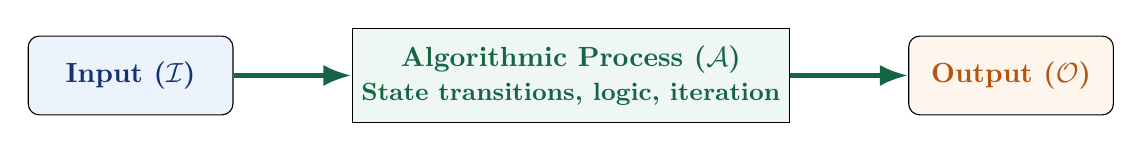
\begin{tikzpicture}[node distance=1.8cm, auto, >=Latex]
    \node [draw, rounded corners, fill=SoftBlue, text=DarkBlue, minimum width=2.6cm, minimum height=1cm, font=\bfseries] (input) {Input ($\mathcal{I}$)};
    \node [draw, rectangle, fill=SoftGreen, text=ForestGreen, minimum width=5.5cm, minimum height=1.2cm, font=\bfseries, right=1.5cm of input, align=center] (algo) {Algorithmic Process ($\mathcal{A}$)\\ \small State transitions, logic, iteration};
    \node [draw, rounded corners, fill=SoftOrange, text=DarkOrange, minimum width=2.6cm, minimum height=1cm, font=\bfseries, right=1.5cm of algo] (output) {Output ($\mathcal{O}$)};
    
    \draw [->, ultra thick, ForestGreen] (input) -- (algo);
    \draw [->, ultra thick, ForestGreen] (algo) -- (output);
\end{tikzpicture}
\end{center}

\subsection{Algorithms versus Programs}
A common beginner mistake is conflating an \emph{algorithm} with a \emph{computer program}. An algorithm represents the abstract mathematical idea and logical workflow, whereas a program is a concrete realization written in a specific language (e.g., Python, C++, Java) executable by hardware.

\begin{center}
\begin{tabularx}{\textwidth}{p{3.2cm} X X}
\toprule
\textbf{Dimension} & \textbf{Algorithm} & \textbf{Program} \\
\midrule
\textbf{Nature} & Conceptual idea, mathematical process & Concrete linguistic implementation \\
\textbf{Language} & Universal, syntax-independent (pseudocode/math) & Python, C++, Rust, Java, etc. \\
\textbf{Level of Detail} & High-level logic, invariants, convergence & Low-level syntax, types, memory, libraries \\
\textbf{Target Audience} & Human mathematicians, software engineers & Translators (compilers, interpreters), CPUs \\
\textbf{Lifespan} & Decades or centuries (e.g., Euclid's GCD: 300 BC) & Subject to library deprecation and syntax changes \\
\bottomrule
\end{tabularx}
\end{center}

\subsection{Essential Characteristics of a Valid Algorithm}
According to Donald Knuth (\emph{The Art of Computer Programming}), every valid computational algorithm must satisfy six core criteria:

\begin{enumerate}[leftmargin=2em, itemsep=3pt]
    \item \textbf{Definiteness (Unambiguity):} Each instruction must be clear, precise, and have exactly one possible interpretation. Ambiguous directives such as ``pick a large number'' or ``sort the items quickly'' are strictly invalid.
    \item \textbf{Defined Input:} An algorithm has zero or more formally specified inputs, each with well-defined domains, data types, and structural preconditions.
    \item \textbf{Defined Output:} An algorithm must produce at least one output or measurable effect that has a specified relationship to the input.
    \item \textbf{Finiteness:} The algorithm must terminate after a finite number of discrete operations for any valid input. Infinite loops violating termination conditions do not constitute algorithms.
    \item \textbf{Effectiveness (Feasibility):} Every operation must be primitive enough that it could, in principle, be executed exactly by a person using paper and pencil in a finite amount of time (e.g., basic integer arithmetic, pointer dereference).
    \item \textbf{Correctness:} For all valid input instances, the algorithm produces the correct output as defined by the specification.
\end{enumerate}

\begin{notebox}[Determinism versus Randomization]
Classical algorithms are \textbf{deterministic}: given an identical input, the algorithm follows the identical execution trajectory and produces identical output. However, modern computer science embraces \textbf{randomized algorithms} (e.g., Randomized QuickSort, Monte Carlo and Las Vegas algorithms) which make random choices during execution. Randomized algorithms remain genuine algorithms provided their probability distribution, termination guarantees, and correctness metrics are rigorously characterized.
\end{notebox}

\subsection{Representation of Algorithms}
Algorithms are communicated across three primary levels of abstraction:
\begin{enumerate}[leftmargin=2em, itemsep=2pt]
    \item \textbf{Natural Language:} Intuitive and accessible, but inherently prone to linguistic ambiguity, verbosity, and lack of formal structural control.
    \item \textbf{Flowcharts:} Visual diagrams utilizing standardized ANSI symbols (Ovals for Start/End, Parallelograms for Input/Output, Rectangles for Processing, and Diamonds for Decision branching). Excellent for visual branching logic, but unmanageable for large systems.
    \item \textbf{Pseudocode:} A structured, high-level informal notation that resembles programming language constructs while omitting syntax overhead (such as semicolons, memory management, and library imports). Pseudocode is the gold standard in academic literature.
\end{enumerate}

\begin{center}
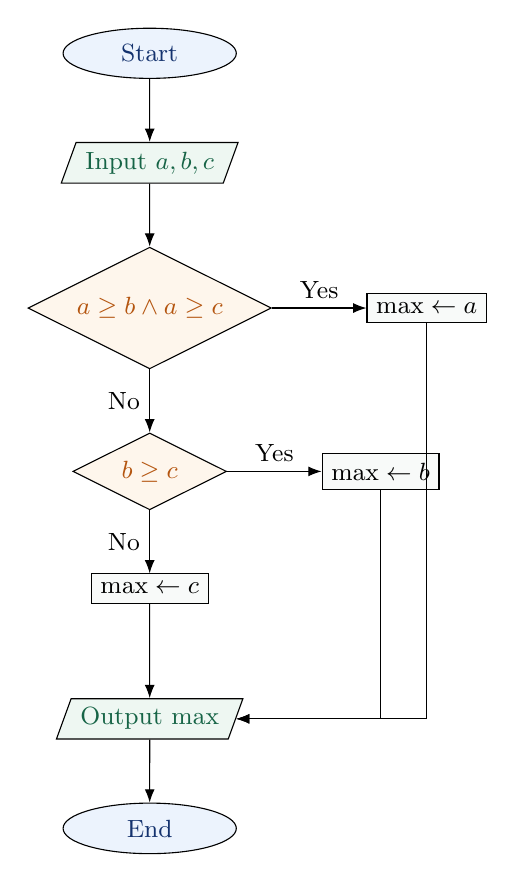
\begin{tikzpicture}[node distance=1.2cm, >=Latex, font=\small]
    \node [draw, ellipse, fill=SoftBlue, text=DarkBlue, minimum width=2.2cm] (start) {Start};
    \node [draw, trapezium, trapezium left angle=70, trapezium right angle=110, fill=SoftGreen, text=ForestGreen, below=0.8cm of start] (in) {Input $a, b, c$};
    \node [draw, diamond, aspect=2, fill=SoftOrange, text=DarkOrange, below=0.8cm of in] (cond1) {$a \ge b \land a \ge c$};
    \node [draw, rectangle, fill=CodeBg, right=1.2cm of cond1] (setA) {$\text{max} \leftarrow a$};
    \node [draw, diamond, aspect=2, fill=SoftOrange, text=DarkOrange, below=0.8cm of cond1] (cond2) {$b \ge c$};
    \node [draw, rectangle, fill=CodeBg, right=1.2cm of cond2] (setB) {$\text{max} \leftarrow b$};
    \node [draw, rectangle, fill=CodeBg, below=0.8cm of cond2] (setC) {$\text{max} \leftarrow c$};
    \node [draw, trapezium, trapezium left angle=70, trapezium right angle=110, fill=SoftGreen, text=ForestGreen, below=1.2cm of setC] (out) {Output max};
    \node [draw, ellipse, fill=SoftBlue, text=DarkBlue, minimum width=2.2cm, below=0.8cm of out] (end) {End};

    \draw [->] (start) -- (in);
    \draw [->] (in) -- (cond1);
    \draw [->] (cond1) -- node[above]{Yes} (setA);
    \draw [->] (cond1) -- node[left]{No} (cond2);
    \draw [->] (cond2) -- node[above]{Yes} (setB);
    \draw [->] (cond2) -- node[left]{No} (setC);
    \draw [->] (setA) |- (out);
    \draw [->] (setB) |- (out);
    \draw [->] (setC) -- (out);
    \draw [->] (out) -- (end);
\end{tikzpicture}
\end{center}

\subsection{The 8-Stage Engineering Workflow for Algorithm Design}
Developing robust computational solutions requires a systematic discipline:
\begin{enumerate}[leftmargin=2.2em, itemsep=2pt]
    \item \textbf{Stage 1: Problem Definition.} Clearly identify what mathematical mapping is needed.
    \item \textbf{Stage 2: Input Specification.} Define parameter domains, scale boundaries ($n \le 10^5$), and data formats.
    \item \textbf{Stage 3: Output Specification.} Define exact return values or side effects.
    \item \textbf{Stage 4: Constraint Identification.} Note real-world constraints (e.g., $O(n \log n)$ time budget, $O(1)$ extra space).
    \item \textbf{Stage 5: Conceptual Formulation.} Devise algorithmic paradigms (Divide-and-Conquer, Greedy, Dynamic Programming).
    \item \textbf{Stage 6: Formal Pseudocode \& Invariants.} Detail loop logic, base cases, and invariants.
    \item \textbf{Stage 7: Edge-Case Verification.} Rigorously test degenerate cases (empty arrays, duplicates, singletons, extreme values).
    \item \textbf{Stage 8: Theoretical Complexity Analysis.} Establish a priori bounds for time and auxiliary space.
\end{enumerate}

\subsection{A Priori versus A Posteriori Analysis}
Evaluating performance is performed through two complementary methodologies:

\begin{center}
\begin{tabularx}{\textwidth}{p{3.5cm} X X}
\toprule
\textbf{Criterion} & \textbf{A Priori Analysis (Theoretical)} & \textbf{A Posteriori Analysis (Empirical)} \\
\midrule
\textbf{Phase} & Before software implementation & After implementation on physical hardware \\
\textbf{Method} & Mathematical counting \& asymptotic bounds & Profiling, CPU timers (`timeit`), memory profilers \\
\textbf{Hardware Dependence} & \textbf{Zero} (Independent of CPU, OS, compiler) & \textbf{High} (Dependent on CPU cache, RAM speed, OS) \\
\textbf{Goal} & Categorize asymptotic growth rate as $n \to \infty$ & Measure exact wall-clock runtime (seconds, MB) \\
\textbf{Representation} & Big-$O$, Big-$\Omega$, Big-$\Theta$ expressions & Plots of milliseconds versus sample size $N$ \\
\bottomrule
\end{tabularx}
\end{center}

\subsection{Why Wall-Clock Time Fails as a Theoretical Metric}
Beginners often ask: \emph{``Why not just measure runtime in seconds using a timer?''} Wall-clock timing is fundamentally flawed for theoretical classification because:
\begin{itemize}[itemsep=1pt]
    \item Runtimes fluctuate wildly across hardware generations (a modern laptop vs. an embedded microcontroller).
    \item Compiler optimizations (vectorization, loop unrolling) alter execution constants by an order of magnitude.
    \item Operating system scheduling, background processes, and cache misses introduce non-deterministic noise.
    \item A program running in $0.001$ seconds on $n = 10$ may take $10^{15}$ years when $n = 100$ if its complexity is $O(2^n)$.
\end{itemize}
Therefore, theoretical analysis counts \textbf{basic machine operations} as a function of the input size $n$.

\newpage
% =========================================================================
\section{Asymptotic Notations and Formal Complexity Foundations}
% =========================================================================

\subsection{The Philosophy of Asymptotics: Focus on Growth Rates}
Asymptotic analysis investigates the behavior of an algorithm's resource consumption (running time $T(n)$ or auxiliary memory $S(n)$) as the input size $n$ approaches infinity ($n \to \infty$). Under this regime, two fundamental simplifications hold:
\begin{enumerate}[itemsep=1pt]
    \item \textbf{Multiplicative Constants are Suppressed:} Whether an algorithm takes $2n$ or $50n$ operations, both scale linearly.
    \item \textbf{Lower-Order Terms are Neglected:} In $f(n) = 3n^2 + 1000n + 50000$, when $n = 10^6$, the quadratic term is $3 \times 10^{12}$ while $1000n = 10^9$ (less than $0.04\%$). The highest-order term dictates scalability.
\end{enumerate}

\subsection{The Three Fundamental Asymptotic Notations}

\begin{definitionbox}[Definition 2.1 (Big $O$ -- Asymptotic Upper Bound)]
Let $f(n)$ and $g(n)$ be functions mapping $\mathbb{N} \to \mathbb{R}^+$. We write:
\[
f(n) = O(g(n)) \quad \text{or} \quad f(n) \in O(g(n))
\]
if and only if there exist strictly positive constants $c > 0$ and $n_0 \ge 1$ such that:
\[
0 \le f(n) \le c \cdot g(n) \quad \text{for all } n \ge n_0.
\]
\textbf{Intuition:} $g(n)$ represents an asymptotic ceiling. The algorithm will perform \emph{at most} proportional to $g(n)$ steps for sufficiently large inputs. Big-$O$ characterizes \textbf{worst-case guarantees}.
\end{definitionbox}

\begin{definitionbox}[Definition 2.2 (Big $\Omega$ -- Asymptotic Lower Bound)]
We write $f(n) = \Omega(g(n))$ if and only if there exist positive constants $c > 0$ and $n_0 \ge 1$ such that:
\[
0 \le c \cdot g(n) \le f(n) \quad \text{for all } n \ge n_0.
\]
\textbf{Intuition:} $g(n)$ provides an asymptotic floor. The algorithm requires \emph{at least} proportional to $g(n)$ steps. Big-$\Omega$ characterizes problem lower bounds (e.g., comparison sort requires $\Omega(n \log n)$).
\end{definitionbox}

\begin{definitionbox}[Definition 2.3 (Big $\Theta$ -- Asymptotically Tight Bound)]
We write $f(n) = \Theta(g(n))$ if and only if there exist positive constants $c_1, c_2 > 0$ and $n_0 \ge 1$ such that:
\[
0 \le c_1 \cdot g(n) \le f(n) \le c_2 \cdot g(n) \quad \text{for all } n \ge n_0.
\]
\textbf{Theorem:} $f(n) = \Theta(g(n)) \iff f(n) = O(g(n)) \text{ and } f(n) = \Omega(g(n))$.
\end{definitionbox}

\begin{center}
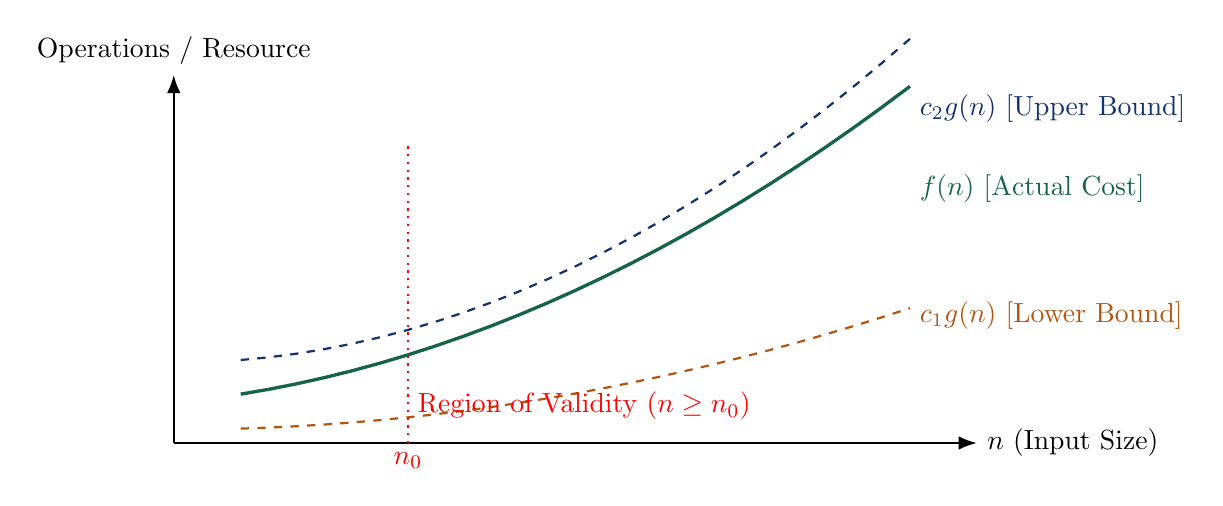
\begin{tikzpicture}[scale=0.85, >=Latex]
    % Axes
    \draw [->, thick] (0,0) -- (12,0) node [right] {$n$ (Input Size)};
    \draw [->, thick] (0,0) -- (0,5.5) node [above] {Operations / Resource};
    
    % Curves
    \draw [dashed, thick, DarkBlue] plot [domain=1:11] (\x, {0.04*\x*\x + 1.2});
    \node [right, DarkBlue] at (11, 5.0) {$c_2 g(n)$ [Upper Bound]};
    
    \draw [very thick, ForestGreen] plot [domain=1:11] (\x, {0.03*\x*\x + 0.1*\x + 0.6});
    \node [right, ForestGreen] at (11, 3.8) {$f(n)$ [Actual Cost]};

    \draw [dashed, thick, DarkOrange] plot [domain=1:11] (\x, {0.015*\x*\x + 0.2});
    \node [right, DarkOrange] at (11, 1.9) {$c_1 g(n)$ [Lower Bound]};

    % Threshold n0
    \draw [dotted, thick, red] (3.5, 0) -- (3.5, 4.5);
    \node [below, red] at (3.5, 0) {$n_0$};
    \node [above right, red] at (3.5, 0.2) {Region of Validity ($n \ge n_0$)};
\end{tikzpicture}
\end{center}

\subsection{The Limit Criterion for Asymptotic Dominance}
Evaluating constants $c$ and $n_0$ from first principles can be tedious. The \textbf{limit test} using L'H\^opital's rule offers an elegant analytical alternative:
\[
L = \lim_{n \to \infty} \frac{f(n)}{g(n)}
\]
\begin{center}
\begin{tabularx}{\textwidth}{l X l}
\toprule
\textbf{Value of Limit $L$} & \textbf{Asymptotic Relationship} & \textbf{Interpretation} \\
\midrule
$L = 0$ & $f(n) = o(g(n))$ and $f(n) = O(g(n))$, but $f(n) \neq \Theta(g(n))$ & $f$ grows strictly slower than $g$ \\
$0 < L < \infty$ & $f(n) = \Theta(g(n))$ (hence also $O(g(n))$ and $\Omega(g(n))$) & $f$ and $g$ have identical growth rates \\
$L = \infty$ & $f(n) = \omega(g(n))$ and $f(n) = \Omega(g(n))$, but $f(n) \neq \Theta(g(n))$ & $f$ grows strictly faster than $g$ \\
\bottomrule
\end{tabularx}
\end{center}

\subsection{Standard Hierarchy of Complexity Classes}
In asymptotic order of growth, common complexity classes are strictly ordered as follows:
\[
O(1) \prec O(\log \log n) \prec O(\log n) \prec O(\sqrt{n}) \prec O(n) \prec O(n \log n) \prec O(n^2) \prec O(n^3) \prec O(2^n) \prec O(n!) \prec O(n^n)
\]

\begin{center}
\begin{tabularx}{\textwidth}{l l p{6.5cm}}
\toprule
\textbf{Class} & \textbf{Formal Name} & \textbf{Canonical Algorithmic Example} \\
\midrule
$O(1)$ & Constant & Array element index access (`arr[i]`), hash table lookup (average) \\
$O(\log \log n)$ & Double Logarithmic & Interpolation search on uniformly distributed data, Van Emde Boas trees \\
$O(\log n)$ & Logarithmic & Binary search in sorted array, balanced BST lookup (AVL, Red-Black) \\
$O(\sqrt{n})$ & Sub-linear & Square root decomposition (Mo's algorithm), trial division primality \\
$O(n)$ & Linear & Linear search, single array traversal, finding min/max \\
$O(n \log n)$ & Linearithmic & Optimal comparison sort (MergeSort, HeapSort, QuickSort avg) \\
$O(n^2)$ & Quadratic & Nested comparison sorts (Bubble, Selection, Insertion), all-pairs checks \\
$O(n^3)$ & Cubic & Naive matrix multiplication ($n \times n$), Floyd-Warshall all-pairs shortest path \\
$O(2^n)$ & Exponential & Generating all subsets (power set), recursive Fibonacci without memoization \\
$O(n!)$ & Factorial & Generating all permutations of $n$ elements, naive Traveling Salesperson \\
\bottomrule
\end{tabularx}
\end{center}

\subsection{Fundamental Operational Rules for Asymptotic Arithmetic}
\begin{enumerate}[leftmargin=2em]
    \item \textbf{Sum Rule (Sequential Blocks):} If code block 1 takes $O(f(n))$ and subsequent block 2 takes $O(g(n))$:
    \[
    T(n) = O(f(n) + g(n)) = O(\max(f(n), g(n)))
    \]
    \item \textbf{Product Rule (Nested Loops):} If an outer loop executes $f(n)$ times and for each step the inner loop performs $g(n)$ operations:
    \[
    T(n) = O(f(n) \cdot g(n))
    \]
    \item \textbf{Scalar Multiplication Invariance:} For any positive constant $k > 0$, $O(k \cdot f(n)) = O(f(n))$.
    \item \textbf{Transitivity:} If $f(n) = O(g(n))$ and $g(n) = O(h(n))$, then $f(n) = O(h(n))$.
\end{enumerate}

\subsection{Space Complexity versus Auxiliary Space}
A precise distinction must be maintained when discussing memory utilization:
\begin{itemize}[itemsep=2pt]
    \item \textbf{Total Space Complexity:} The complete memory allocated by the program, which equals $\text{Input Space} + \text{Auxiliary Space}$.
    \item \textbf{Auxiliary Space:} The \emph{extra or temporary} storage created by the algorithm during its execution to solve the problem (excluding the memory required to hold the inputs).
\end{itemize}

\begin{examplebox}[Auxiliary Space in Recursion: The Call Stack]
A recursive implementation of factorial allocates no auxiliary arrays:
\begin{lstlisting}[style=pythonstyle]
def factorial(n):
    if n <= 1:
        return 1
    return n * factorial(n - 1)
\end{lstlisting}
Although no user variables are allocated, each recursive call places an \textbf{activation record} (call frame containing return address, local parameters, and saved registers) onto the runtime call stack. Since the call stack reaches depth $n$, the \textbf{auxiliary space is $\Theta(n)$}.
\end{examplebox}

\newpage
% =========================================================================
\section{In-Depth Code \& Loop Complexity Analysis}
% =========================================================================

\subsection{Linear Increment Loops: $\Theta(n)$}
When the loop control variable is incremented or decremented by a non-zero constant $c$:
\begin{lstlisting}[style=pythonstyle]
i = 0
while i < n:
    # O(1) body operations
    i += c
\end{lstlisting}
The number of iterations is $k = \lceil n / c \rceil$. By dropping constant factors, $T(n) = \Theta(n)$.

\subsection{Logarithmic Loops (Multiplication / Division): $\Theta(\log n)$}
When the loop variable is multiplied or divided by a constant factor $b > 1$:
\begin{lstlisting}[style=pythonstyle]
i = 1
while i < n:
    # O(1) body operations
    i *= 2
\end{lstlisting}
At iteration $k$, the variable has value $i = 2^k$. The loop terminates when $2^k \ge n \implies k = \lceil \log_2 n \rceil$. Thus, $T(n) = \Theta(\log n)$. Note that by the logarithm change-of-base rule ($\log_b n = \frac{\ln n}{\ln b}$), the base of the logarithm only contributes a constant factor, so we write $O(\log n)$ without specifying the base.

\subsection{Triangular Nested Loops: $\Theta(n^2)$}
When the inner loop boundary depends directly on the outer loop index:
\begin{lstlisting}[style=pythonstyle]
for i in range(n):
    for j in range(i, n):
        # O(1) constant operation
        process(i, j)
\end{lstlisting}
The inner loop executes $n - i$ times. The total operations sum as:
\[
S(n) = \sum_{i=0}^{n-1} (n - i) = n + (n-1) + (n-2) + \dots + 1 = \frac{n(n+1)}{2} = \frac{1}{2}n^2 + \frac{1}{2}n
\]
Neglecting lower-order terms and the scalar coefficient $\frac{1}{2}$, the running time is $\Theta(n^2)$.

\subsection{Geometric Series Loop Progressions: $\Theta(n)$}
Consider the following nested structure where the outer variable halves and the inner loop runs linearly up to the outer index:
\begin{lstlisting}[style=pythonstyle]
def geometric_loop(n):
    i = n
    while i > 0:
        for j in range(i):
            print(j)
        i //= 2
\end{lstlisting}
\textbf{Mathematical Analysis:} The outer loop takes values $i = n, \lfloor n/2 \rfloor, \lfloor n/4 \rfloor, \dots, 1$. The total operation count is bounded by an infinite geometric series:
\[
S(n) = n + \frac{n}{2} + \frac{n}{4} + \frac{n}{8} + \dots \le n \sum_{k=0}^{\infty} \left(\frac{1}{2}\right)^k = n \cdot \frac{1}{1 - 1/2} = 2n
\]
Since $S(n) \le 2n$, the time complexity is strictly $\Theta(n)$, \textbf{not} $O(n \log n)$.

\subsection{Harmonic Number Loops: $\Theta(n \log n)$}
Consider a loop pattern frequently encountered in prime sieving (Sieve of Eratosthenes):
\begin{lstlisting}[style=pythonstyle]
for i in range(1, n + 1):
    j = i
    while j <= n:
        # O(1) step
        j += i
\end{lstlisting}
For each $i$, the inner loop executes $\lfloor n / i \rfloor$ times. The total count is:
\[
T(n) = \sum_{i=1}^n \left\lfloor \frac{n}{i} \right\rfloor \approx n \sum_{i=1}^n \frac{1}{i} = n \cdot H_n
\]
where $H_n = 1 + \frac{1}{2} + \frac{1}{3} + \dots + \frac{1}{n} = \ln n + \gamma + O(1/n)$ is the $n$-th Harmonic Number. Therefore, $T(n) = \Theta(n \log n)$.

\subsection{Quadratic Loop Conditions: $\Theta(\sqrt{n})$}
\begin{lstlisting}[style=pythonstyle]
i = 1
while i * i <= n:
    # O(1) operations
    i += 1
\end{lstlisting}
The loop condition $i^2 \le n$ is mathematically equivalent to $i \le \sqrt{n}$. The loop executes $\lfloor \sqrt{n} \rfloor$ times, yielding time complexity $\Theta(\sqrt{n})$.

\subsection{Best-Case, Worst-Case, and Average-Case Behavior}
Algorithmic complexity often depends on the arrangement of input data:
\begin{itemize}[itemsep=2pt]
    \item \textbf{Best Case ($T_{\text{best}}(n)$):} The minimum number of operations required across any input instance of size $n$. For Linear Search, finding the target at index $0$ takes $\Omega(1)$ time.
    \item \textbf{Worst Case ($T_{\text{worst}}(n)$):} The maximum operations across any input instance of size $n$. For Linear Search, scanning the entire array when the item is absent takes $O(n)$ time.
    \item \textbf{Average Case ($T_{\text{avg}}(n)$):} The expected number of operations assuming a uniform probability distribution over all possible input permutations. For Linear Search:
    \[
    T_{\text{avg}}(n) = \sum_{i=1}^n \frac{1}{n} \cdot i = \frac{1}{n} \frac{n(n+1)}{2} = \frac{n+1}{2} = \Theta(n)
    \]
\end{itemize}

\newpage
% =========================================================================
\section{Divide-and-Conquer Recurrences and the Master Theorem}
% =========================================================================

\subsection{Formulating Recurrence Relations}
Divide-and-conquer algorithms partition a problem of size $n$ into $a$ smaller subproblems, each of size $n/b$, solve them recursively, and merge the partial solutions with combining cost $f(n)$. The general recurrence relation is:
\[
T(n) = a T\left(\frac{n}{b}\right) + f(n)
\]
\begin{itemize}[itemsep=1pt]
    \item $a \ge 1$: Number of subproblems solved recursively at each level.
    \item $b > 1$: Factor by which the input size is reduced in each subproblem.
    \item $f(n)$: Cost of dividing the input and combining results outside the recursive calls.
\end{itemize}

\subsection{The Recursion Tree Method}
The recursion tree provides complete structural insight into how work accumulates across recursive levels:

\begin{center}
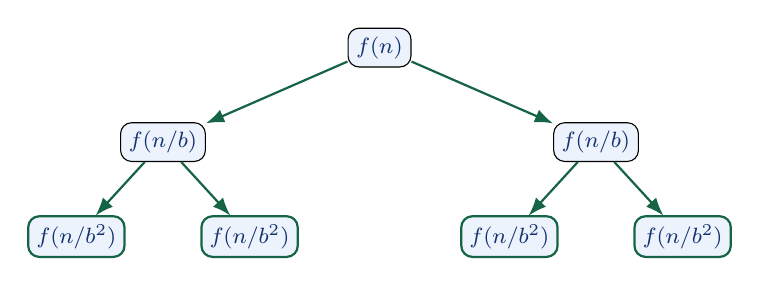
\begin{tikzpicture}[
    level 1/.style={sibling distance=5.5cm, level distance=1.2cm},
    level 2/.style={sibling distance=2.2cm, level distance=1.2cm},
    every node/.style={draw, rounded corners, fill=SoftBlue, text=DarkBlue, font=\footnotesize, inner sep=3pt},
    edge from parent/.style={draw, -Latex, thick, ForestGreen}
]
    \node {$f(n)$}
        child { node {$f(n/b)$}
            child { node {$f(n/b^2)$} }
            child { node {$f(n/b^2)$} }
        }
        child { node {$f(n/b)$}
            child { node {$f(n/b^2)$} }
            child { node {$f(n/b^2)$} }
        };
\end{tikzpicture}
\end{center}

\begin{enumerate}[leftmargin=2em, itemsep=2pt]
    \item \textbf{Tree Depth:} Subproblem size at level $j$ is $n/b^j$. The base case is reached when $n/b^j = 1 \implies \text{Depth } D = \log_b n$.
    \item \textbf{Number of Subproblems at Level $j$:} Exactly $a^j$ nodes.
    \item \textbf{Total Leaves at Depth $\log_b n$:} $a^{\log_b n} = n^{\log_b a}$ leaves.
    \item \textbf{Leaf-Level Cost:} If base cases cost $\Theta(1)$, total leaf cost is $\Theta(n^{\log_b a})$.
\end{enumerate}

\subsection{The Standard Master Theorem (CLRS)}

\begin{theorembox}[Theorem 4.1 (Master Theorem for Divide-and-Conquer)]
Let $a \ge 1$ and $b > 1$ be constants, let $f(n)$ be an asymptotically positive function, and let $T(n)$ be defined on the integers by $T(n) = a T(n/b) + f(n)$. The asymptotic behavior of $T(n)$ is determined by comparing $f(n)$ to the watershed function $n^{\log_b a}$:

\begin{itemize}[leftmargin=1.5em, itemsep=4pt]
    \item \textbf{Case 1 (Leaf Dominant -- Recursion Dominates):}
    If there exists a constant $\epsilon > 0$ such that:
    \[
    f(n) = O\left(n^{\log_b a - \epsilon}\right)
    \]
    then $f(n)$ is polynomially smaller than $n^{\log_b a}$, and:
    \[
    T(n) = \Theta\left(n^{\log_b a}\right)
    \]

    \item \textbf{Case 2 (Balanced Work Distribution):}
    If $f(n) = \Theta\left(n^{\log_b a}\right)$, the cost is evenly distributed across all $\log_b n$ levels:
    \[
    T(n) = \Theta\left(n^{\log_b a} \log n\right)
    \]

    \item \textbf{Case 3 (Root Dominant -- Combine Cost Dominates):}
    If there exists a constant $\epsilon > 0$ such that $f(n) = \Omega\left(n^{\log_b a + \epsilon}\right)$, and if $f(n)$ satisfies the \textbf{regularity condition}:
    \[
    a \cdot f(n/b) \le c \cdot f(n) \quad \text{for some constant } c < 1 \text{ and all sufficiently large } n,
    \]
    then:
    \[
    T(n) = \Theta(f(n))
    \]
\end{itemize}
\end{theorembox}

\begin{notebox}[The Requirement of a Polynomial Gap]
In Cases 1 and 3, the difference between $f(n)$ and $n^{\log_b a}$ must be \textbf{polynomial} (a factor of $n^\epsilon$ for $\epsilon > 0$), not merely logarithmic. For example, in $T(n) = 2T(n/2) + n / \log n$, we have $n^{\log_2 2} = n$. The function $f(n) = n / \log n$ is asymptotically smaller than $n$, but the gap is $1/\log n$, which is sub-polynomial ($n^\epsilon > \log n$ for any $\epsilon > 0$). Hence, the standard 3-case Master Theorem cannot solve this recurrence.
\end{notebox}

\subsection{The Extended Master Theorem (Polylogarithmic Form)}
To resolve recurrences with logarithmic factors in $f(n)$, computer scientists utilize the extended formulation:

\begin{theorembox}[Theorem 4.2 (Extended Master Theorem)]
For recurrences of the form $T(n) = a T(n/b) + \Theta(n^k \log^p n)$ with $a \ge 1, b > 1, k \ge 0$, compare $a$ with $b^k$:

\begin{center}
\begin{tabularx}{\textwidth}{l l X}
\toprule
\textbf{Condition} & \textbf{Log Exponent $p$} & \textbf{Solution $T(n)$} \\
\midrule
$a > b^k$ & Any $p \in \mathbb{R}$ & $\Theta\left(n^{\log_b a}\right)$ \hfill (Recursion dominates) \\
\midrule
\multirow{3}{*}{$a = b^k$} & $p > -1$ & $\Theta\left(n^k \log^{p+1} n\right)$ \hfill (Standard balanced) \\
& $p = -1$ & $\Theta\left(n^k \log \log n\right)$ \hfill (Boundary logarithmic case) \\
& $p < -1$ & $\Theta\left(n^k\right)$ \hfill (Sum converges) \\
\midrule
$a < b^k$ & $p \ge 0$ & $\Theta\left(n^k \log^p n\right)$ \hfill (Root cost dominates) \\
& $p < 0$ & $O\left(n^k\right)$ \\
\bottomrule
\end{tabularx}
\end{center}
\end{theorembox}

\subsection{When the Master Theorem Cannot Be Applied (7 Classic Traps)}
The Master Theorem is powerful, but fails when:
\begin{enumerate}[itemsep=2pt]
    \item \textbf{Variable Subproblem Count:} $a$ is not a constant (e.g., $T(n) = 2^n T(n/2) + n^n$).
    \item \textbf{Non-Uniform Subproblem Sizes:} Subproblems have varying fractions (e.g., $T(n) = T(n/3) + T(2n/3) + n$). Requires Akra-Bazzi method or recursion tree.
    \item \textbf{Sub-Polynomial Gap:} In $T(n) = 2T(n/2) + n/\log n$, Case 1 fails because $n/\log n$ is not $O(n^{1-\epsilon})$.
    \item \textbf{Subproblem Fraction $b \le 1$:} Subproblem sizes decrease by subtraction, not division (e.g., $T(n) = T(n-1) + n$).
    \item \textbf{Violation of Regularity:} In Case 3, $f(n)$ oscillates or fails $a f(n/b) \le c f(n)$ (e.g., $T(n) = 2T(n/2) + n^2 (2 + \cos n)$).
    \item \textbf{Subproblem Count $a < 1$:} For example, $T(n) = 0.5 T(n/2) + 1/n$.
    \item \textbf{Non-Positive Combining Function:} $f(n)$ takes negative values (e.g., $T(n) = 64T(n/8) - n^2 \log n$).
\end{enumerate}

\subsection{Subtract-and-Conquer Recurrences}
When problem size decreases by a fixed subtraction amount $b > 0$:
\[
T(n) = a T(n - b) + f(n), \quad \text{where } f(n) = O(n^k)
\]
\begin{center}
\begin{tabularx}{\textwidth}{l X l}
\toprule
\textbf{Condition on $a$} & \textbf{Complexity $T(n)$} & \textbf{Representative Example} \\
\midrule
$a < 1$ & $O(f(n)) = O(n^k)$ & $T(n) = 0.5 T(n-1) + n^2 \implies O(n^2)$ \\
$a = 1$ & $O(n \cdot f(n)) = O(n^{k+1})$ & $T(n) = T(n-1) + n \implies O(n^2)$ (Selection Sort) \\
$a > 1$ & $O(f(n) \cdot a^{n/b}) = O(n^k a^{n/b})$ & $T(n) = 2 T(n-1) + 1 \implies O(2^n)$ (Towers of Hanoi) \\
\bottomrule
\end{tabularx}
\end{center}

\subsection{Advanced Recurrences via Variable Substitution}
\begin{examplebox}[Solving $T(n) = \sqrt{n} \cdot T(\sqrt{n}) + n$]
This recurrence cannot be solved by the Master Theorem because $a = \sqrt{n}$ is not constant.
\begin{enumerate}
    \item Divide both sides by $n$:
    \[
    \frac{T(n)}{n} = \frac{\sqrt{n} \cdot T(\sqrt{n})}{n} + 1 = \frac{T(\sqrt{n})}{\sqrt{n}} + 1
    \]
    \item Define substitution variable $U(n) = \frac{T(n)}{n}$. The relation becomes:
    \[
    U(n) = U(\sqrt{n}) + 1
    \]
    \item Track input shrinkage: $n \to n^{1/2} \to n^{1/4} \to \dots \to n^{1/2^k}$.
    \item The process terminates when subproblem size reaches a constant $c = 2$:
    \[
    n^{1/2^k} = 2 \implies \frac{1}{2^k} \log_2 n = 1 \implies 2^k = \log_2 n \implies k = \log_2(\log_2 n)
    \]
    \item Each step adds $1$, so $U(n) = \Theta(\log \log n)$.
    \item Re-substituting $T(n) = n \cdot U(n)$ yields:
    \[
    T(n) = \Theta(n \log \log n)
    \]
\end{enumerate}
\end{examplebox}

\newpage
% =========================================================================
\section{Amortized Analysis Foundations \& Case Studies}
% =========================================================================

\subsection{The Motivation for Amortized Analysis}
Traditional worst-case analysis evaluates the maximum cost of an individual operation in isolation. However, in many sophisticated data structures:
\begin{itemize}[itemsep=1pt]
    \item An expensive operation cannot occur in isolation; it requires a long sequence of prior cheap operations to set up.
    \item Evaluating every operation by the worst-case single step produces an overly pessimistic bound.
\end{itemize}

\begin{definitionbox}[Definition 5.1 (Amortized Cost)]
In a sequence of $m$ operations, if the worst-case total running time across the entire sequence is $T(m)$, the \textbf{amortized cost} per operation is:
\[
\hat{c} = \frac{T(m)}{m}
\]
\textbf{Key Distinction:} Amortized analysis guarantees an upper bound on the average performance of each operation in the \emph{worst-case sequence}. It involves \textbf{no probabilistic assumptions} about the input distribution (unlike average-case analysis).
\end{definitionbox}

\subsection{The Three Standard Amortized Analysis Techniques}

\subsubsection{1. The Aggregate Method}
Show that for all $m$, a sequence of $m$ operations takes total time $T(m)$ in the worst case. The amortized cost per operation is directly computed as $\hat{c} = T(m) / m$.

\subsubsection{2. The Accounting Method (Banker's Method)}
Assign an artificial charge (\textbf{amortized cost} $\hat{c}_i$) to each operation type:
\begin{itemize}[itemsep=1pt]
    \item Cheap operations are overcharged ($\hat{c}_i > c_i$), and the surplus is stored as ``credit'' on specific data structure elements.
    \item Expensive operations are undercharged ($\hat{c}_i < c_i$), and draw from the accumulated credit to pay for their actual cost.
    \item \textbf{Validity Invariant:} Total stored credit must remain non-negative at all times:
    \[
    \sum_{i=1}^m \hat{c}_i \ge \sum_{i=1}^m c_i \quad \text{for all } m \ge 1.
    \]
\end{itemize}

\subsubsection{3. The Potential Method (Physicist's Method)}
Define a \textbf{potential function} $\Phi(D)$ mapping the data structure state $D$ to a real number $\mathbb{R}$:
\begin{itemize}[itemsep=1pt]
    \item $\Phi(D_0) = 0$ (initial state potential is 0).
    \item $\Phi(D_i) \ge 0$ for all valid states $D_i$ (potential is always non-negative).
    \item The amortized cost of the $i$-th operation is defined as:
    \[
    \hat{c}_i = c_i + \Phi(D_i) - \Phi(D_{i-1}) = c_i + \Delta\Phi_i
    \]
    \item Summing across all $m$ operations telescopes the potential terms:
    \[
    \sum_{i=1}^m \hat{c}_i = \sum_{i=1}^m \left(c_i + \Phi(D_i) - \Phi(D_{i-1})\right) = \sum_{i=1}^m c_i + \Phi(D_m) - \Phi(D_0) \ge \sum_{i=1}^m c_i
    \]
\end{itemize}

\subsection{Case Study 1: Dynamic Array (Python `list`) Resizing}
Consider a dynamic array that doubles its capacity whenever an element is appended to a full array:
\begin{lstlisting}[style=pythonstyle]
class DynamicArray:
    def __init__(self):
        self.capacity = 1
        self.size = 0
        self.data = [None] * self.capacity

    def append(self, x):
        if self.size == self.capacity:
            self._resize(2 * self.capacity)
        self.data[self.size] = x
        self.size += 1

    def _resize(self, new_capacity):
        new_data = [None] * new_capacity
        for i in range(self.size):
            new_data[i] = self.data[i]
        self.data = new_data
        self.capacity = new_capacity
\end{lstlisting}

\subsubsection{Analysis via Aggregate Method}
\begin{itemize}[itemsep=2pt]
    \item An insertion that requires no resize costs $1$ operation.
    \item Array expansions occur when $n = 1, 2, 4, 8, 16, \dots, 2^k$.
    \item The total number of element copying operations across $n$ insertions is:
    \[
    \sum_{j=0}^{\lfloor \log_2 n \rfloor} 2^j = 2^{\lfloor \log_2 n \rfloor + 1} - 1 < 2n
    \]
    \item Total cost for $n$ operations is $T(n) = n \text{ (insertions)} + 2n \text{ (copies)} \le 3n$.
    \item \textbf{Amortized Cost:} $\hat{c} = \frac{T(n)}{n} \le \frac{3n}{n} = 3 = \Theta(1)$.
\end{itemize}

\begin{notebox}[Doubling versus Fixed Increments]
If the array increased its capacity by a fixed constant $+k$ (e.g., $+1000$ elements) instead of doubling, an array reaching size $n$ would undergo $\approx n/k$ resizes, copying $\sum_{i=1}^{n/k} i \cdot k \approx \Theta(n^2)$ elements. The amortized cost per append would degrade to $\Theta(n)$! Geometric doubling is mandatory to achieve $O(1)$ amortized insertion.
\end{notebox}

\subsubsection{Analysis via Potential Method}
Let $s_i$ be the number of items and $c_i$ be the capacity after the $i$-th operation. Define the potential function:
\[
\Phi(D_i) = 2 s_i - c_i
\]
\begin{itemize}[itemsep=2pt]
    \item \textbf{Non-negativity:} Immediately after a doubling, $c_i = 2 s_i \implies \Phi(D_i) = 0$. When full, $c_i = s_i \implies \Phi(D_i) = s_i \ge 0$.
    \item \textbf{Case A (No Resize):} $c_i = c_{i-1}$, $s_i = s_{i-1} + 1$.
    \[
    \hat{c}_i = c_i + \Delta\Phi_i = 1 + (2(s_{i-1} + 1) - c_{i-1}) - (2 s_{i-1} - c_{i-1}) = 1 + 2 = 3
    \]
    \item \textbf{Case B (With Resize):} Array was full ($s_{i-1} = c_{i-1}$). New capacity $c_i = 2 c_{i-1}$. Actual cost $c_i = s_{i-1} + 1$.
    \[
    \Delta\Phi_i = (2(s_{i-1} + 1) - 2 s_{i-1}) - (2 s_{i-1} - s_{i-1}) = 2 - s_{i-1}
    \]
    \[
    \hat{c}_i = (s_{i-1} + 1) + (2 - s_{i-1}) = 3
    \]
\end{itemize}
In both cases, $\hat{c}_i = 3 = O(1)$. The amortized cost per append is strictly $O(1)$.

\subsection{Case Study 2: Stack with MultiPop}
Consider a stack data structure with standard `Push(x)` ($O(1)$), `Pop()` ($O(1)$), and `MultiPop(k)` which pops $\min(k, \text{size})$ items:
\begin{lstlisting}[style=pythonstyle]
def multipop(stack, k):
    while stack and k > 0:
        stack.pop()
        k -= 1
\end{lstlisting}
\textbf{Analysis:} A single `MultiPop` operation can cost $O(n)$ if the stack contains $n$ elements. However, an element can only be popped if it was previously pushed. In any sequence of $m$ operations starting with an empty stack, the total number of pops cannot exceed the total number of pushes (which is $\le m$). Hence, total time is at most $2m$, yielding an \textbf{amortized cost of $O(1)$ per operation}.

\newpage
% =========================================================================
\section{Worked Problems and Solutions}
% =========================================================================

\subsection{Problem 1: Growth Rate Ranking}
\textbf{Problem:} Rank the following functions in order of asymptotic growth rate from slowest to fastest. Group functions that belong to the same $\Theta$-class:
\[
f_1(n) = n^{1.5}, \quad f_2(n) = 1000n, \quad f_3(n) = n \log_2 n, \quad f_4(n) = 2^{\sqrt{n}}, \quad f_5(n) = n!, \quad f_6(n) = 2^n, \quad f_7(n) = n^2
\]

\begin{definitionbox}[Solution to Problem 1]
Taking logarithms or evaluating limits:
\begin{enumerate}[itemsep=1pt]
    \item $f_2(n) = 1000n = \Theta(n)$
    \item $f_3(n) = n \log_2 n$ (grows faster than $n$, slower than $n^{1.5}$)
    \item $f_1(n) = n^{1.5} = n^{3/2}$
    \item $f_7(n) = n^2$
    \item $f_4(n) = 2^{\sqrt{n}}$: compare with $n^2$. $\log_2(2^{\sqrt{n}}) = \sqrt{n}$, whereas $\log_2(n^2) = 2 \log_2 n$. Since $\sqrt{n} \succ \log n$, $2^{\sqrt{n}}$ eventually dominates all polynomials! Thus $n^2 \prec 2^{\sqrt{n}} \prec 2^n$.
    \item $f_6(n) = 2^n$
    \item $f_5(n) = n! \approx \sqrt{2\pi n}(n/e)^n$ (Stirling's approximation, dominates $2^n$).
\end{enumerate}
\textbf{Final Ranking:}
\[
1000n \prec n \log n \prec n^{1.5} \prec n^2 \prec 2^{\sqrt{n}} \prec 2^n \prec n!
\]
\end{definitionbox}

\subsection{Problem 2: Non-Trivial Loop Complexity}
\textbf{Problem:} Compute the tight asymptotic bound $\Theta$ for the following Python function:
\begin{lstlisting}[style=pythonstyle]
def compute(n):
    total = 0
    i = 1
    while i <= n:
        j = 1
        while j <= n:
            total += 1
            j *= 2
        i += 1
    return total
\end{lstlisting}

\begin{definitionbox}[Solution to Problem 2]
\begin{itemize}[itemsep=2pt]
    \item The outer loop initializes $i = 1$ and increments $i \leftarrow i + 1$ until $i > n$. Thus, the outer loop executes exactly $n$ times.
    \item For every single outer iteration, the inner loop initializes $j = 1$ and doubles $j \leftarrow j \times 2$ until $j > n$. The sequence of $j$ values is $1, 2, 4, 8, \dots, 2^k$. The inner loop terminates when $2^k > n \implies k = \lfloor \log_2 n \rfloor + 1$. The inner loop executes $\Theta(\log n)$ times independently of $i$.
    \item By the Product Rule: $T(n) = \sum_{i=1}^n \Theta(\log n) = n \cdot \Theta(\log n) = \Theta(n \log n)$.
\end{itemize}
\end{definitionbox}

\subsection{Problem 3: Applying the Master Theorem}
\textbf{Problem:} Solve the following divide-and-conquer recurrence relations:
\begin{enumerate}[itemsep=2pt]
    \item $T_a(n) = 8 T_a(n/2) + n^2$
    \item $T_b(n) = 2 T_b(n/2) + n \log^2 n$
    \item $T_c(n) = 3 T_c(n/4) + n \log n$
\end{enumerate}

\begin{definitionbox}[Solution to Problem 3]
\textbf{Part 1:} For $T_a(n) = 8 T_a(n/2) + n^2$:
\begin{itemize}[itemsep=1pt]
    \item $a = 8, b = 2, f(n) = n^2$.
    \item Benchmark: $n^{\log_b a} = n^{\log_2 8} = n^3$.
    \item Compare $f(n) = n^2$ with $n^3$: Since $n^2 = O(n^{3 - 1})$ with $\epsilon = 1 > 0$, this falls into \textbf{Case 1}.
    \item \textbf{Conclusion:} $T_a(n) = \Theta(n^3)$.
\end{itemize}

\textbf{Part 2:} For $T_b(n) = 2 T_b(n/2) + n \log^2 n$:
\begin{itemize}[itemsep=1pt]
    \item $a = 2, b = 2, f(n) = n \log^2 n$.
    \item Benchmark: $n^{\log_2 2} = n^1$. Here $k = 1$ and $p = 2$.
    \item Since $a = b^k$ ($2 = 2^1$) and $p = 2 > -1$, this falls into \textbf{Extended Case 2}.
    \item \textbf{Conclusion:} $T_b(n) = \Theta(n^k \log^{p+1} n) = \Theta(n \log^3 n)$.
\end{itemize}

\textbf{Part 3:} For $T_c(n) = 3 T_c(n/4) + n \log n$:
\begin{itemize}[itemsep=1pt]
    \item $a = 3, b = 4, f(n) = n \log n$.
    \item Benchmark: $n^{\log_4 3} \approx n^{0.7925}$.
    \item Here $f(n) = n \log n = \Omega(n^{0.7925 + \epsilon})$ for $\epsilon \approx 0.2$.
    \item Regularity check: $a f(n/b) = 3(n/4 \log(n/4)) \le \frac{3}{4} n \log n$. Choosing $c = 0.8 < 1$, regularity holds.
    \item This is \textbf{Case 3}.
    \item \textbf{Conclusion:} $T_c(n) = \Theta(n \log n)$.
\end{itemize}
\end{definitionbox}

\newpage
% =========================================================================
\section{Quick Reference Summary Sheet}
% =========================================================================

\subsection{Essential Summation Formulas}
\begin{itemize}[itemsep=3pt]
    \item \textbf{Arithmetic Series:} $\sum_{i=1}^n i = 1 + 2 + \dots + n = \frac{n(n+1)}{2} = \Theta(n^2)$
    \item \textbf{Sum of Squares:} $\sum_{i=1}^n i^2 = \frac{n(n+1)(2n+1)}{6} = \Theta(n^3)$
    \item \textbf{Finite Geometric Series ($r \neq 1$):} $\sum_{i=0}^k r^i = \frac{r^{k+1} - 1}{r - 1}$
    \item \textbf{Infinite Geometric Series ($|r| < 1$):} $\sum_{i=0}^{\infty} r^i = \frac{1}{1 - r}$
    \item \textbf{Harmonic Series:} $\sum_{i=1}^n \frac{1}{i} = \ln n + \gamma + O(1/n) = \Theta(\log n)$
    \item \textbf{Stirling's Factorial Approximation:} $n! = \sqrt{2\pi n} \left(\frac{n}{e}\right)^n \left(1 + O(1/n)\right) \implies \log(n!) = \Theta(n \log n)$
\end{itemize}

\subsection{Master Theorem Decision Matrix}
For recurrences $T(n) = a T(n/b) + \Theta(n^k \log^p n)$:
\begin{center}
\begin{tabularx}{\textwidth}{c c c X}
\toprule
\textbf{Comparison} & \textbf{Exponent $p$} & \textbf{Dominant Factor} & \textbf{Solution $T(n)$} \\
\midrule
$a > b^k$ & Any $p$ & Leaves ($\text{Depth } \log_b n$) & $\Theta(n^{\log_b a})$ \\
\midrule
$a = b^k$ & $p > -1$ & All Levels Equal & $\Theta(n^k \log^{p+1} n)$ \\
$a = b^k$ & $p = -1$ & Boundary & $\Theta(n^k \log \log n)$ \\
$a = b^k$ & $p < -1$ & Leaf/Root & $\Theta(n^k)$ \\
\midrule
$a < b^k$ & $p \ge 0$ & Root (Combine Cost) & $\Theta(n^k \log^p n)$ \\
$a < b^k$ & $p < 0$ & Root & $O(n^k)$ \\
\bottomrule
\end{tabularx}
\end{center}

\subsection{Amortized Cost Comparison Matrix}
\begin{center}
\begin{tabularx}{\textwidth}{p{3.5cm} p{2.5cm} p{2.5cm} X}
\toprule
\textbf{Operation} & \textbf{Worst-Case} & \textbf{Amortized} & \textbf{Key Mechanism} \\
\midrule
Dynamic Array `append` & $O(n)$ (during resize) & $O(1)$ & Geometric doubling ensures total resize copies $< 2n$ \\
Stack `MultiPop(k)` & $O(k)$ & $O(1)$ & Elements cannot be popped more times than pushed \\
$k$-bit Counter Increment & $O(k)$ & $O(1)$ & Bit $i$ flips once every $2^i$ operations: $\sum 1/2^i \le 2$ \\
Hash Table Insert & $O(n)$ (rehash) & $O(1)$ & Capacity doubling with uniform hash distribution \\
\bottomrule
\end{tabularx}
\end{center}

\vspace{1.5em}
\begin{center}
\rule{0.6\textwidth}{0.6pt}\\[0.4em]
{\small\color{ForestGreen}\textbf{End of Lecture Notes -- Part 03: Algorithms and Complexity Analysis}}\\[0.2em]
{\footnotesize\color{DarkGray}Department of Data Science \& AI $\cdot$ National Economics University}
\end{center}

\end{document}
